% !TEX root = ../partial-sdm.tex

Performance matters --- and has always mattered. If an experiment takes a few seconds, there is no point arguing whether we should try it. If it takes a few hours, maybe we should think first. If it takes a few days, it is more important to make a good plan. As SDM consumes a lot of both processor and memory resources, some experiments may take a long time.

Each scan a 1,000-bits SDM with 1,000,000 hard-locations executes $10^9$ bit compares through $10^9/64 = 15,625,000$ XORs and calls to the built-in popcount. So, 10,000 writes execute $10^{13}$ bit compares, while a 6-iterative reading executes $6 \cdot 10^{12}$ bit compares. The heatmap of Figure \ref{fig:cir-dist-10k-writes-kanerva} executed $3.05 \cdot 10^{15}$ bit compares. For comparison, the number of seconds since Jesus's birth is 63,639,648,000 = $6.36 \cdot 10^{10}$. The number of people who have ever lived on earth is estimated to be $1,08 \cdot 10^{11}$. There are approximtely $1.8 \cdot 10^{9}$ websites in the internet. A modern laptop can increment a counter $5 \cdot 10^{8}$ times per second. Hence, a naive implementation of SDM may take several hours to simply write 10,000 random bitstrings.

Amazon EC2 p3.2xlarge has generated the heatmap of Figure \ref{fig:cir-dist-10k-writes-kanerva} in 15 minutes and 3 seconds. It has compared $3.37 \cdot 10^{12}$ bits per second through $52.6 \cdot 10^{9} = 52.6 \text{ billion}$ XORs and popcounts per second. It is a great improvement when compared to the first versions of the code which took 16 hours to generate the same heatmap (and its memory use was already optimized and the computations were distributed in threads).

We have executed the same performance test in each device. The test has 3 parts. The first part consists of: 1,000 linear scans, 5,000 thread scans, and 5,000 OpenCL scans. The second part consists of 5,000 writes, 5,000 single reads, and 1,000 6-iterative readings, with both thread and opencl scanners. The code is available in the ``Performance test'' notebook \citep{sdmframework}.

Our first device is a personal MacBook Pro Retina 13-inch Late 2013 with a 2.6GHz Intel core i5 processor, 6GB DDR3 RAM, and Intel Iris GPU.

Our second device is an iMac Retina 5K 27-inch 2017 with a 3.8GHz Intel core i5 processor, 8GB DDR4 RAM, and a Radeon Pro 580 8G CPU. The complete results are presented in Figures \ref{fig:perf-imac-read-256}, \ref{fig:perf-imac-write-256}, \ref{fig:perf-imac-read-1000}, \ref{fig:perf-imac-write-1000}, \ref{fig:perf-imac-scan-256}, \ref{fig:perf-imac-scan-1000}, and \ref{fig:perf-imac-scan-10k} and Tables \ref{tab:perf-imac-256}, \ref{tab:perf-imac-1000}, and \ref{tab:perf-imac-10k}.

Beyond that, we are also running in state-of-the-art devices: (i) an Amazon EC2 p2.xlarge with Intel Xeon E5-2686v4 processor, 61GB DDR3 RAM, and NVIDIA K80 GPU, and (ii) an Amazon EC2 p3.2xlarge with Intel Xeon E5-2686v4 processor, 488GB DDR3 RAM, and NVIDIA Tesla V100 GPU.

It is interesting that which scanner is faster depends also on the SDM settings. In the iMac 2017, the faster scanner for a 1,000-bits SDM was the OpenCL, but for a 256-bit SDM was the threads. What happened here is that the OpenCL kernel chosen was a generic one which performs the scan for any SDM. It is always possible to optimize the OpenCL kernel to a specific setting, and it would be faster than the threads. By default, the framework chooses a generic kernel which we believe would be reasonable for the most common setups.
% TODO Run the optimized kernel and show the results.

Most of the time, the bottleneck of both the read and the write operations is the scanner. But we have optimized the OpenCL kernel so much for the iMac 2017 that scanner not the bottleneck anymore. In the writing operation, it took the same time to scan and to update the counters. It is impressive because it update, on average, 1,000 counters of 32-bit integers each, and it was as fast as (i) sending the command to the GPU, (ii) performing 1 billion bit compares, and (iii) downloading the response from the GPU.

Our conclusion is that, if one is really concerned about performance, one should fine tune the OpenCL kernel for one's GPU. It would always be faster than running in the CPU.


Kernel comparisons

\begin{table}[!htb]
\centering
\begin{tabular}{| l | r | r | r |}
    \hline
    & Loops & Scans / second & Scan time (ms) \\ \hline
    single\_scan0 & 3000 & 15.02 & 199.62 & 5.00 \\
    single\_scan1 & 3000 & 11.87 & 252.64 & 3.95 \\
    single\_scan2 & 3000 & 13.73 & 218.38 & 4.57 \\
    single\_scan3 & 3000 & 11.06 & 271.15 & 3.68 \\
    single\_scan4 & 3000 & 12.13 & 247.28 & 4.04 \\
    single\_scan5 & 3000 & 11.18 & 268.29 & 3.72 \\
    single\_scan5\_unroll & 3000 & 10.84 & 276.70 & 3.6139983336130777 \\
    single\_scan6 & 3000 & 12.08 & 248.26 & 4.02 \\
    \hline
\end{tabular}
\caption{iMac Retina 5K 27-inch 2017 with a 3.8GHz Intel core i5 processor, 8GB DDR4 RAM, and a Radeon Pro 580 8G GPU. Running an SDM with $n=1,000$ bits, $H=1,000,000$, and $r=451$.
\label{tab:perf-imac-256}}
\end{table}

\begin{table}[!htb]
\centering
\begin{tabular}{| l | r | r | r |}
    \hline
    & Loops & Scans / second & Scan time (ms) \\ \hline
    single\_scan0 & 3000 & 9.09 & 329.71 & 3.03 \\
    single\_scan1 & 3000 & 8.63 & 347.42 & 2.87 \\
    single\_scan2 & 3000 & 11.46 & 261.73 & 3.82 \\
    single\_scan3 & 3000 & 11.18 & 268.16 & 3.72 \\
    single\_scan4 & 3000 & 13.44 & 223.18 & 4.48 \\
    single\_scan5 & 3000 & 11.29 & 265.59 & 3.76 \\
    single\_scan5\_unroll & 3000 & 11.39 & 263.24 & 3.79 \\
    single\_scan6 & 3000 & 13.10 & 228.92 & 4.36 \\
\end{tabular}
\caption{iMac Retina 5K 27-inch 2017 with a 3.8GHz Intel core i5 processor, 8GB DDR4 RAM, and a Radeon Pro 580 8G GPU. Running an SDM with $n=256$ bits, $H=1,000,000$, and $r=103$.
\label{tab:perf-imac-256}}
\end{table}

\begin{table}[!htb]
\centering
\begin{tabular}{| l | r | r | r |}
    \hline
    & Loops & Scans / second & Scan time (ms) \\ \hline
    single\_scan0 & 500 & 30.53 & 16.37 & 61.06 \\
    single\_scan1 & 500 & 22.48 & 22.24 & 44.96 \\
    single\_scan2 & 500 & 22.49 & 22.23 & 44.98 \\
    single\_scan3 & 500 & 6.33 & 78.92 & 12.67 \\
    single\_scan4 & 500 & 5.72 & 87.30 & 11.45 \\
    single\_scan5 & 500 & 6.29 & 79.43 & 12.58 \\
    single\_scan5\_unroll & 500 & 5.68 & 87.88 & 11.37 \\
    single\_scan6 & 500 & 5.48 & 91.21 & 10.96 \\
\end{tabular}
\caption{iMac Retina 5K 27-inch 2017 with a 3.8GHz Intel core i5 processor, 8GB DDR4 RAM, and a Radeon Pro 580 8G GPU. Running an SDM with $n=10,000$ bits, $H=1,000,000$, and $r=4850$.
\label{tab:perf-imac-256}}
\end{table}

\begin{table}[!htb]
\centering
\begin{tabular}{| l | r | r | r |}
    \hline
    & Loops & Scans / second & Scan time (ms) \\ \hline
    single\_scan0 & 1000 & 23.60 & 42.36 & 23.60 \\
    single\_scan1 & 1000 & 13.22 & 75.63 & 13.22 \\
    single\_scan2 & 1000 & 47.28 & 21.14 & 47.28 \\
    single\_scan3 & 1000 & 33.06 & 30.24 & 33.06 \\
    single\_scan4 & 1000 & 40.32 & 24.79 & 40.32 \\
    single\_scan5 & 1000 & 31.51 & 31.73 & 31.51 \\
    single\_scan5\_unroll & 1000 & 27.55 & 36.28 & 27.55 \\
    single\_scan6 & 1000 & 39.48 & 25.32 & 39.48 \\
\end{tabular}
\caption{MacBook Pro Retina 13-inch Late 2013 with a 2.6GHz Intel core i5 processor, 6GB DDR3 RAM, and Intel Iris GPU. Running an SDM with $n=1,000$ bits, $H=1,000,000$, and $r=451$.
\label{tab:perf-imac-256}}
\end{table}

\begin{table}[!htb]
\centering
\begin{tabular}{| l | r | r | r |}
    \hline
    & Loops & Scans / second & Scan time (ms) \\ \hline
    single\_scan0 & 1000 & 8.36 & 119.49 & 8.36 \\
    single\_scan1 & 1000 & 10.43 & 95.82 & 10.43 \\
    single\_scan2 & 1000 & 23.48 & 42.58 & 23.48 \\
    single\_scan3 & 1000 & 25.51 & 39.19 & 25.51 \\
    single\_scan4 & 1000 & 42.39 & 23.58 & 42.39 \\
    single\_scan5 & 1000 & 24.42 & 40.94 & 24.42 \\
    single\_scan5\_unroll & 1000 & 22.77 & 43.91 & 22.77 \\
    single\_scan6 & 1000 & 42.18 & 23.70 & 42.18 \\
\end{tabular}
\caption{MacBook Pro Retina 13-inch Late 2013 with a 2.6GHz Intel core i5 processor, 6GB DDR3 RAM, and Intel Iris GPU. Running an SDM with $n=256$ bits, $H=1,000,000$, and $r=103$.
\label{tab:perf-imac-256}}
\end{table}

\begin{table}[!htb]
\centering
\begin{tabular}{| l | r | r | r |}
    \hline
    & Loops & Scans / second & Scan time (ms) \\ \hline
    Loops & Total time & Scans per second & Time per scan (ms) \\
    single\_scan0 & 3000 & 2.09 & 1433.27 & 0.69 \\
    single\_scan1 & 3000 & 1.64 & 1822.51 & 0.54 \\
    single\_scan2 & 3000 & 2.57 & 1165.06 & 0.85 \\
    single\_scan3 & 3000 & 3.06 & 979.93 & 1.02 \\
    single\_scan4 & 3000 & 3.30 & 906.35 & 1.10 \\
    single\_scan5 & 3000 & 2.85 & 1049.21 & 0.95 \\
    single\_scan6 & 3000 & 3.12 & 958.50 & 1.04 \\
\end{tabular}
\caption{EC2 p3.2xlarge 1000 bits
\label{tab:perf-imac-256}}
\end{table}

\begin{table}[!htb]
\centering
\begin{tabular}{| l | r | r | r |}
    \hline
    & Loops & Scans / second & Scan time (ms) \\ \hline
    Loops & Total time & Scans per second & Time per scan (ms) \\
    single\_scan0 & 3000 & 1.09 & 2729.58 & 0.36 \\
    single\_scan1 & 3000 & 1.10 & 2703.49 & 0.36 \\
    single\_scan2 & 3000 & 2.21 & 1354.12 & 0.73 \\
    single\_scan3 & 3000 & 1.90 & 1573.43 & 0.63 \\
    single\_scan4 & 3000 & 3.15 & 951.22 & 1.05 \\
    single\_scan5 & 3000 & 1.87 & 1598.69 & 0.62 \\
    single\_scan6 & 3000 & 3.04 & 986.06 & 1.01 \\
\end{tabular}
\caption{EC2 p3.2xlarge 256 bits
\label{tab:perf-imac-256}}
\end{table}

\begin{table}[!htb]
\centering
\begin{tabular}{| l | r | r | r |}
    \hline
    & Loops & Scans / second & Scan time (ms) \\ \hline
    Loops & Total time & Scans per second & Time per scan (ms) \\
    single\_scan0 & 500 & 10.30 & 48.54 & 20.60 \\
    single\_scan1 & 500 & 2.47 & 202.34 & 4.94 \\
    single\_scan2 & 500 & 2.50 & 199.29 & 5.01 \\
    single\_scan3 & 500 & 3.03 & 164.66 & 6.07 \\
    single\_scan4 & 500 & 2.99 & 166.70 & 5.99 \\
    single\_scan5 & 500 & 2.68 & 186.26 & 5.36 \\
    single\_scan6 & 500 & 2.98 & 167.74 & 5.96 \\
\end{tabular}
\caption{EC2 p3.2xlarge 10k bits
\label{tab:perf-imac-256}}
\end{table}

\begin{table}[!htb]
\centering
\begin{tabular}{| l | r | r | r |}
    \hline
    & Loops & Scans / second & Scan time (ms) \\ \hline
    Loops & Total time & Scans per second & Time per scan (ms) \\
    single\_scan0 & 3000 & 11.38 & 263.61 & 3.79 \\
    single\_scan1 & 3000 & 11.83 & 253.45 & 3.94 \\
    single\_scan2 & 3000 & 25.62 & 117.06 & 8.54 \\
    single\_scan3 & 3000 & 29.21 & 102.70 & 9.73 \\
    single\_scan4 & 3000 & 34.15 & 87.82 & 11.38 \\
    single\_scan5 & 3000 & 29.86 & 100.46 & 9.95 \\
    single\_scan6 & 3000 & 34.00 & 88.21 & 11.33 \\
\end{tabular}
\caption{EC2 p2.xlarge 1000 bits
\label{tab:perf-imac-256}}
\end{table}

\begin{table}[!htb]
\centering
\begin{tabular}{| l | r | r | r |}
    \hline
    & Loops & Scans / second & Scan time (ms) \\ \hline
    Loops & Total time & Scans per second & Time per scan (ms) \\
    single\_scan0 & 3000 & 2.28 & 1312.85 & 0.76 \\
    single\_scan1 & 3000 & 2.42 & 1237.20 & 0.80 \\
    single\_scan2 & 3000 & 16.77 & 178.85 & 5.59 \\
    single\_scan3 & 3000 & 18.93 & 158.43 & 6.31 \\
    single\_scan4 & 3000 & 30.88 & 97.14 & 10.29 \\
    single\_scan5 & 3000 & 20.07 & 149.45 & 6.69 \\
    single\_scan6 & 3000 & 30.89 & 97.10 & 10.29 \\
\end{tabular}
\caption{EC2 p2.xlarge 256 bits
\label{tab:perf-imac-256}}
\end{table}

\begin{table}[!htb]
\centering
\begin{tabular}{| l | r | r | r |}
    \hline
    & Loops & Scans / second & Scan time (ms) \\ \hline
    Loops & Total time & Scans per second & Time per scan (ms) \\
    single\_scan0 & 500 & 17.72 & 28.20 & 35.45 \\
    single\_scan1 & 500 & 28.90 & 17.30 & 57.80 \\
    single\_scan2 & 500 & 31.85 & 15.69 & 63.71 \\
    single\_scan3 & 500 & 19.96 & 25.04 & 39.92 \\
    single\_scan4 & 500 & 22.74 & 21.97 & 45.49 \\
    single\_scan5 & 500 & 21.75 & 22.97 & 43.51 \\
    single\_scan6 & 500 & 20.71 & 24.13 & 41.42 \\
\end{tabular}
\caption{EC2 p2.xlarge 10k bits
\label{tab:perf-imac-256}}
\end{table}

\begin{figure}[!htb]
\centering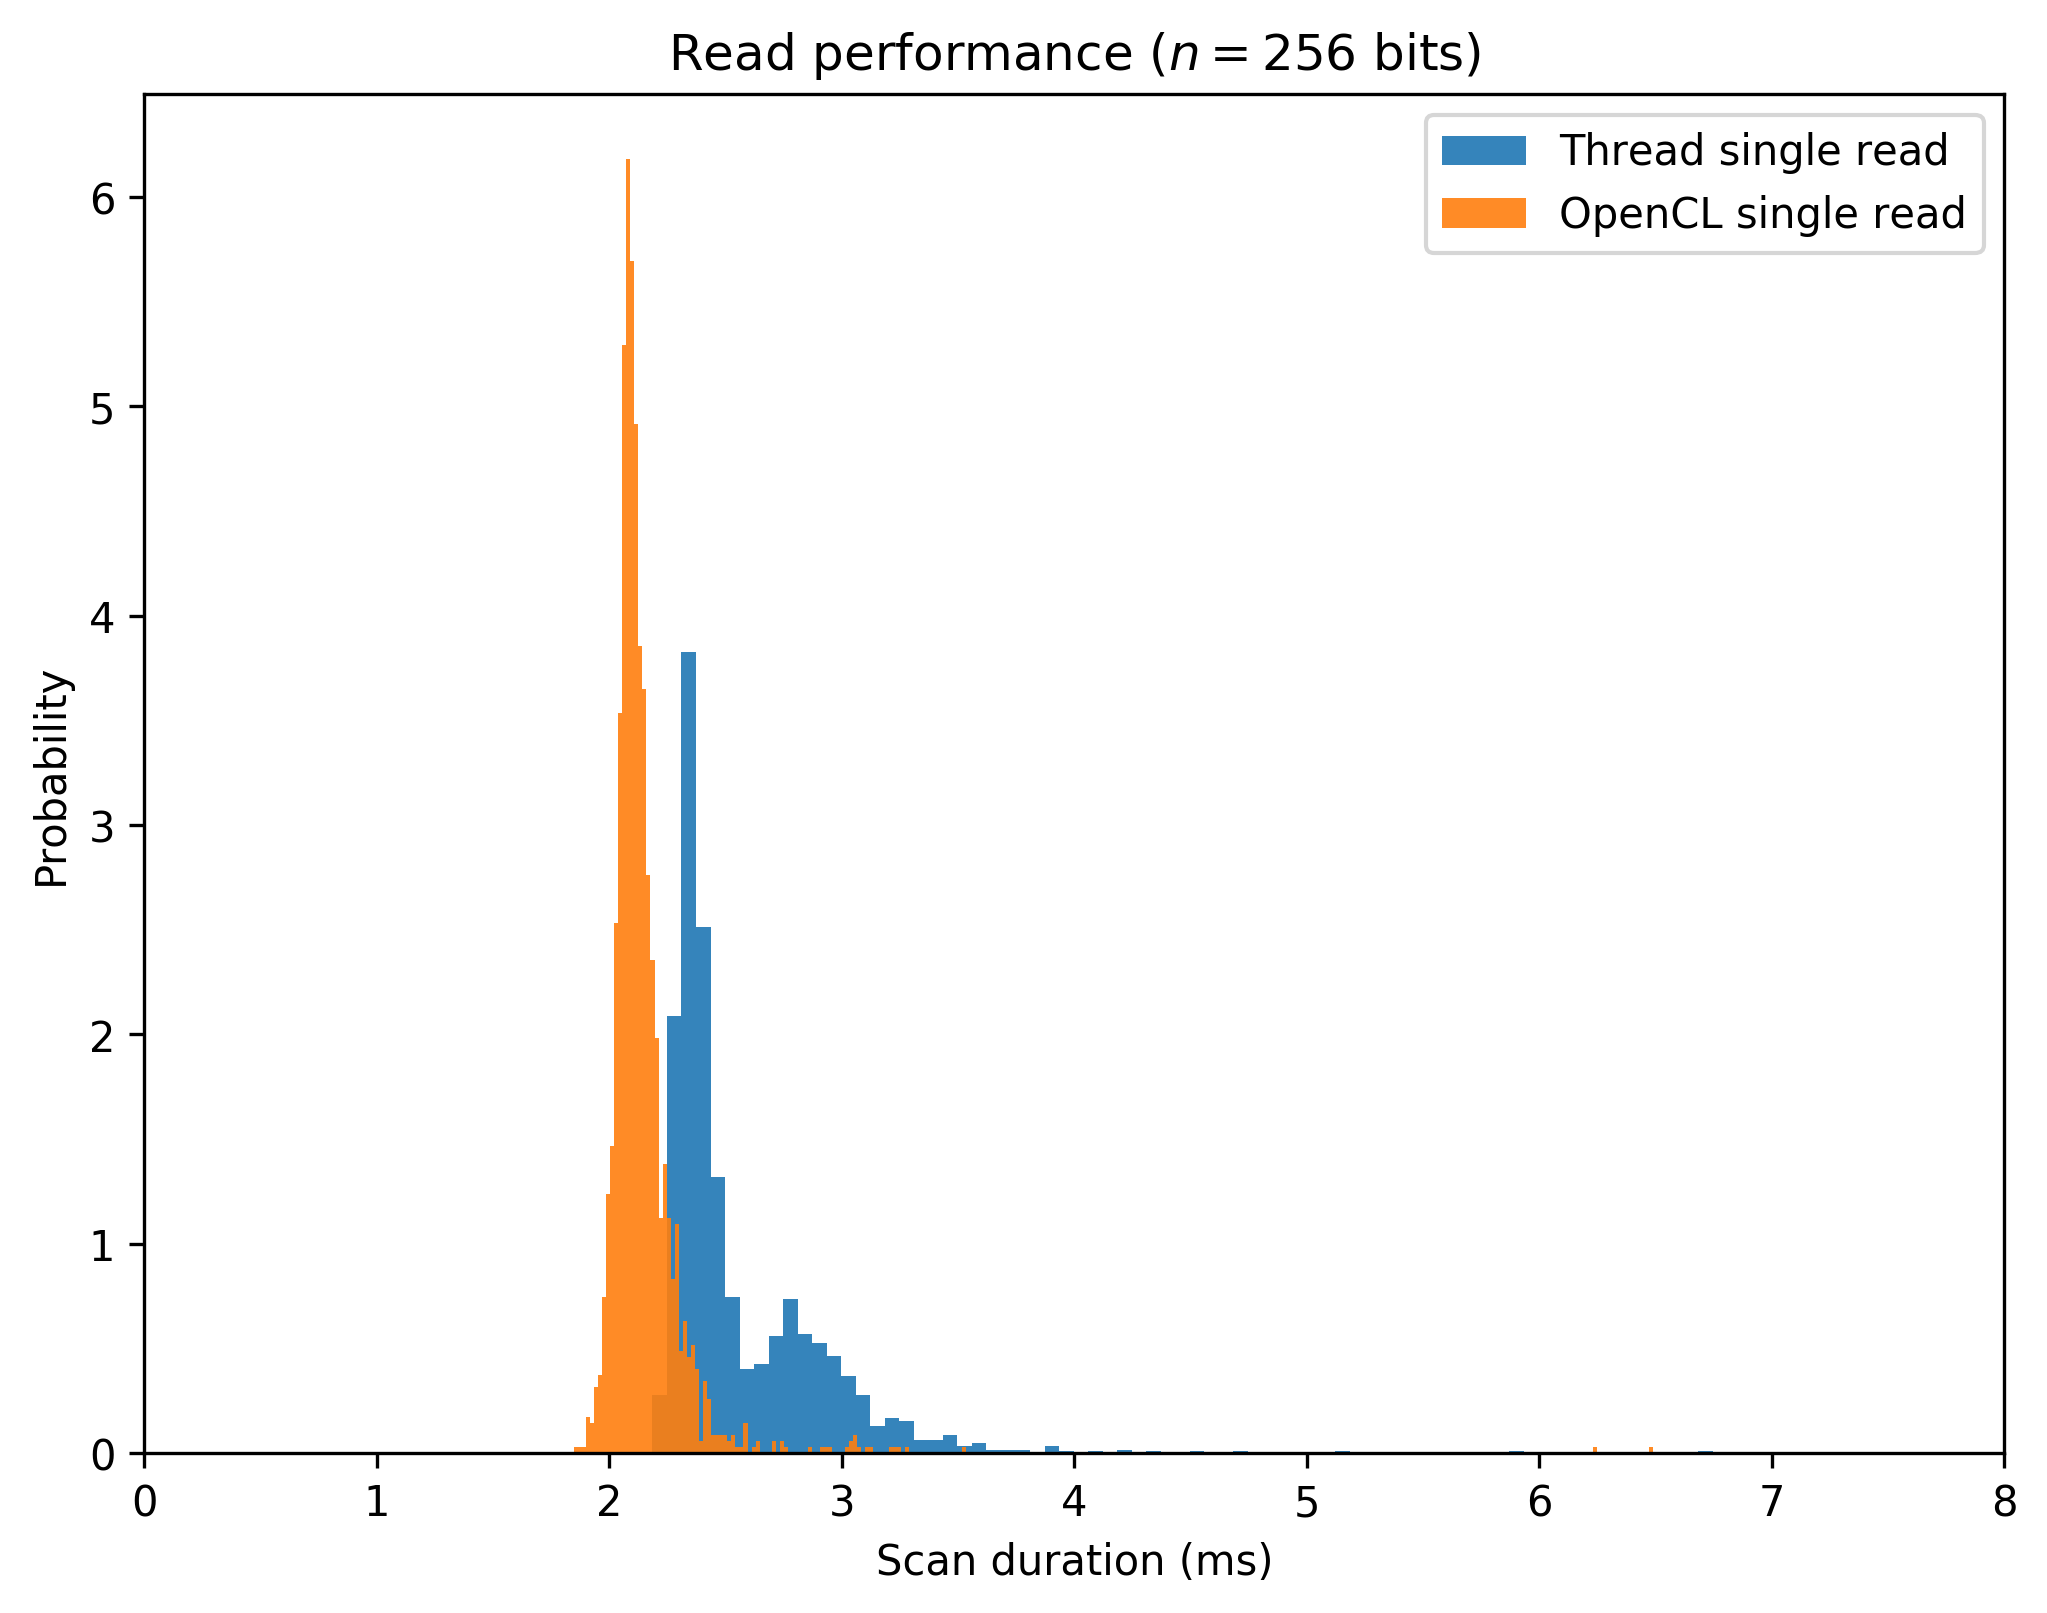
\includegraphics[width=\textwidth]{images02/performance/imac-read-256.png}
\caption{Time to run a single read in a SDM with $n=256$, $H=1,000,000$ and $r=103$.
\label{fig:perf-imac-read-256}}
\end{figure}

\begin{figure}[!htb]
\centering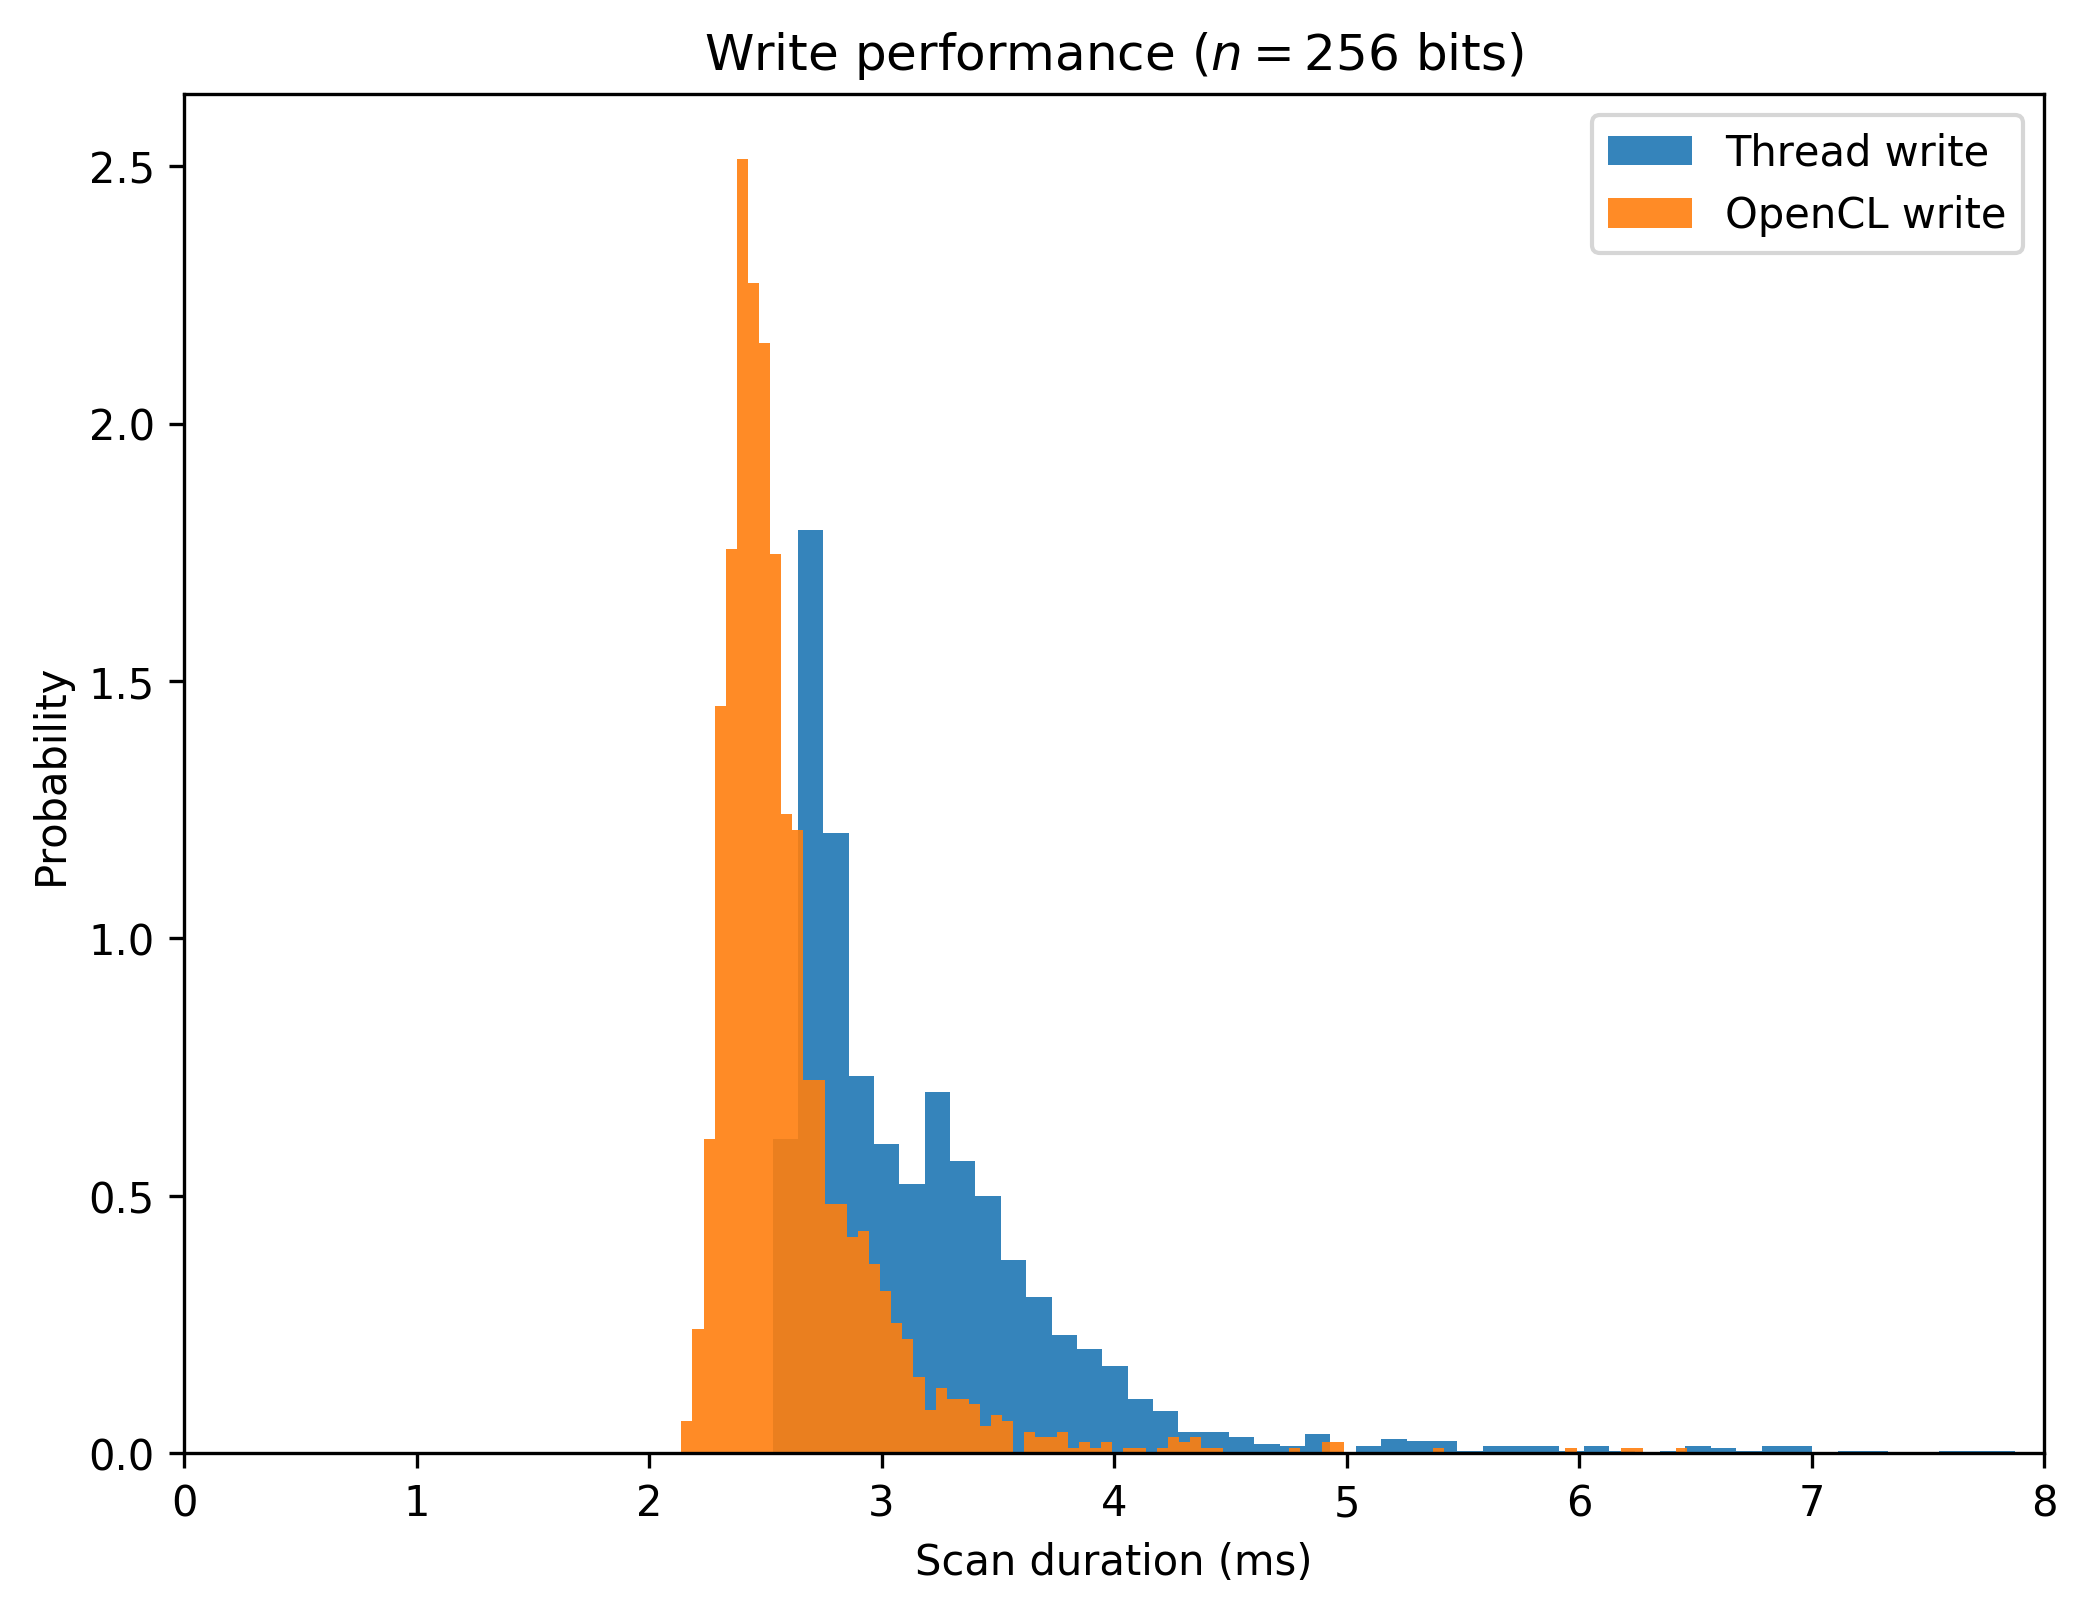
\includegraphics[width=\textwidth]{images02/performance/imac-write-256.png}
\caption{Time to run one write in a SDM with $n=256$, $H=1,000,000$ and $r=103$.
\label{fig:perf-imac-write-256}}
\end{figure}

\begin{figure}[!htb]
\centering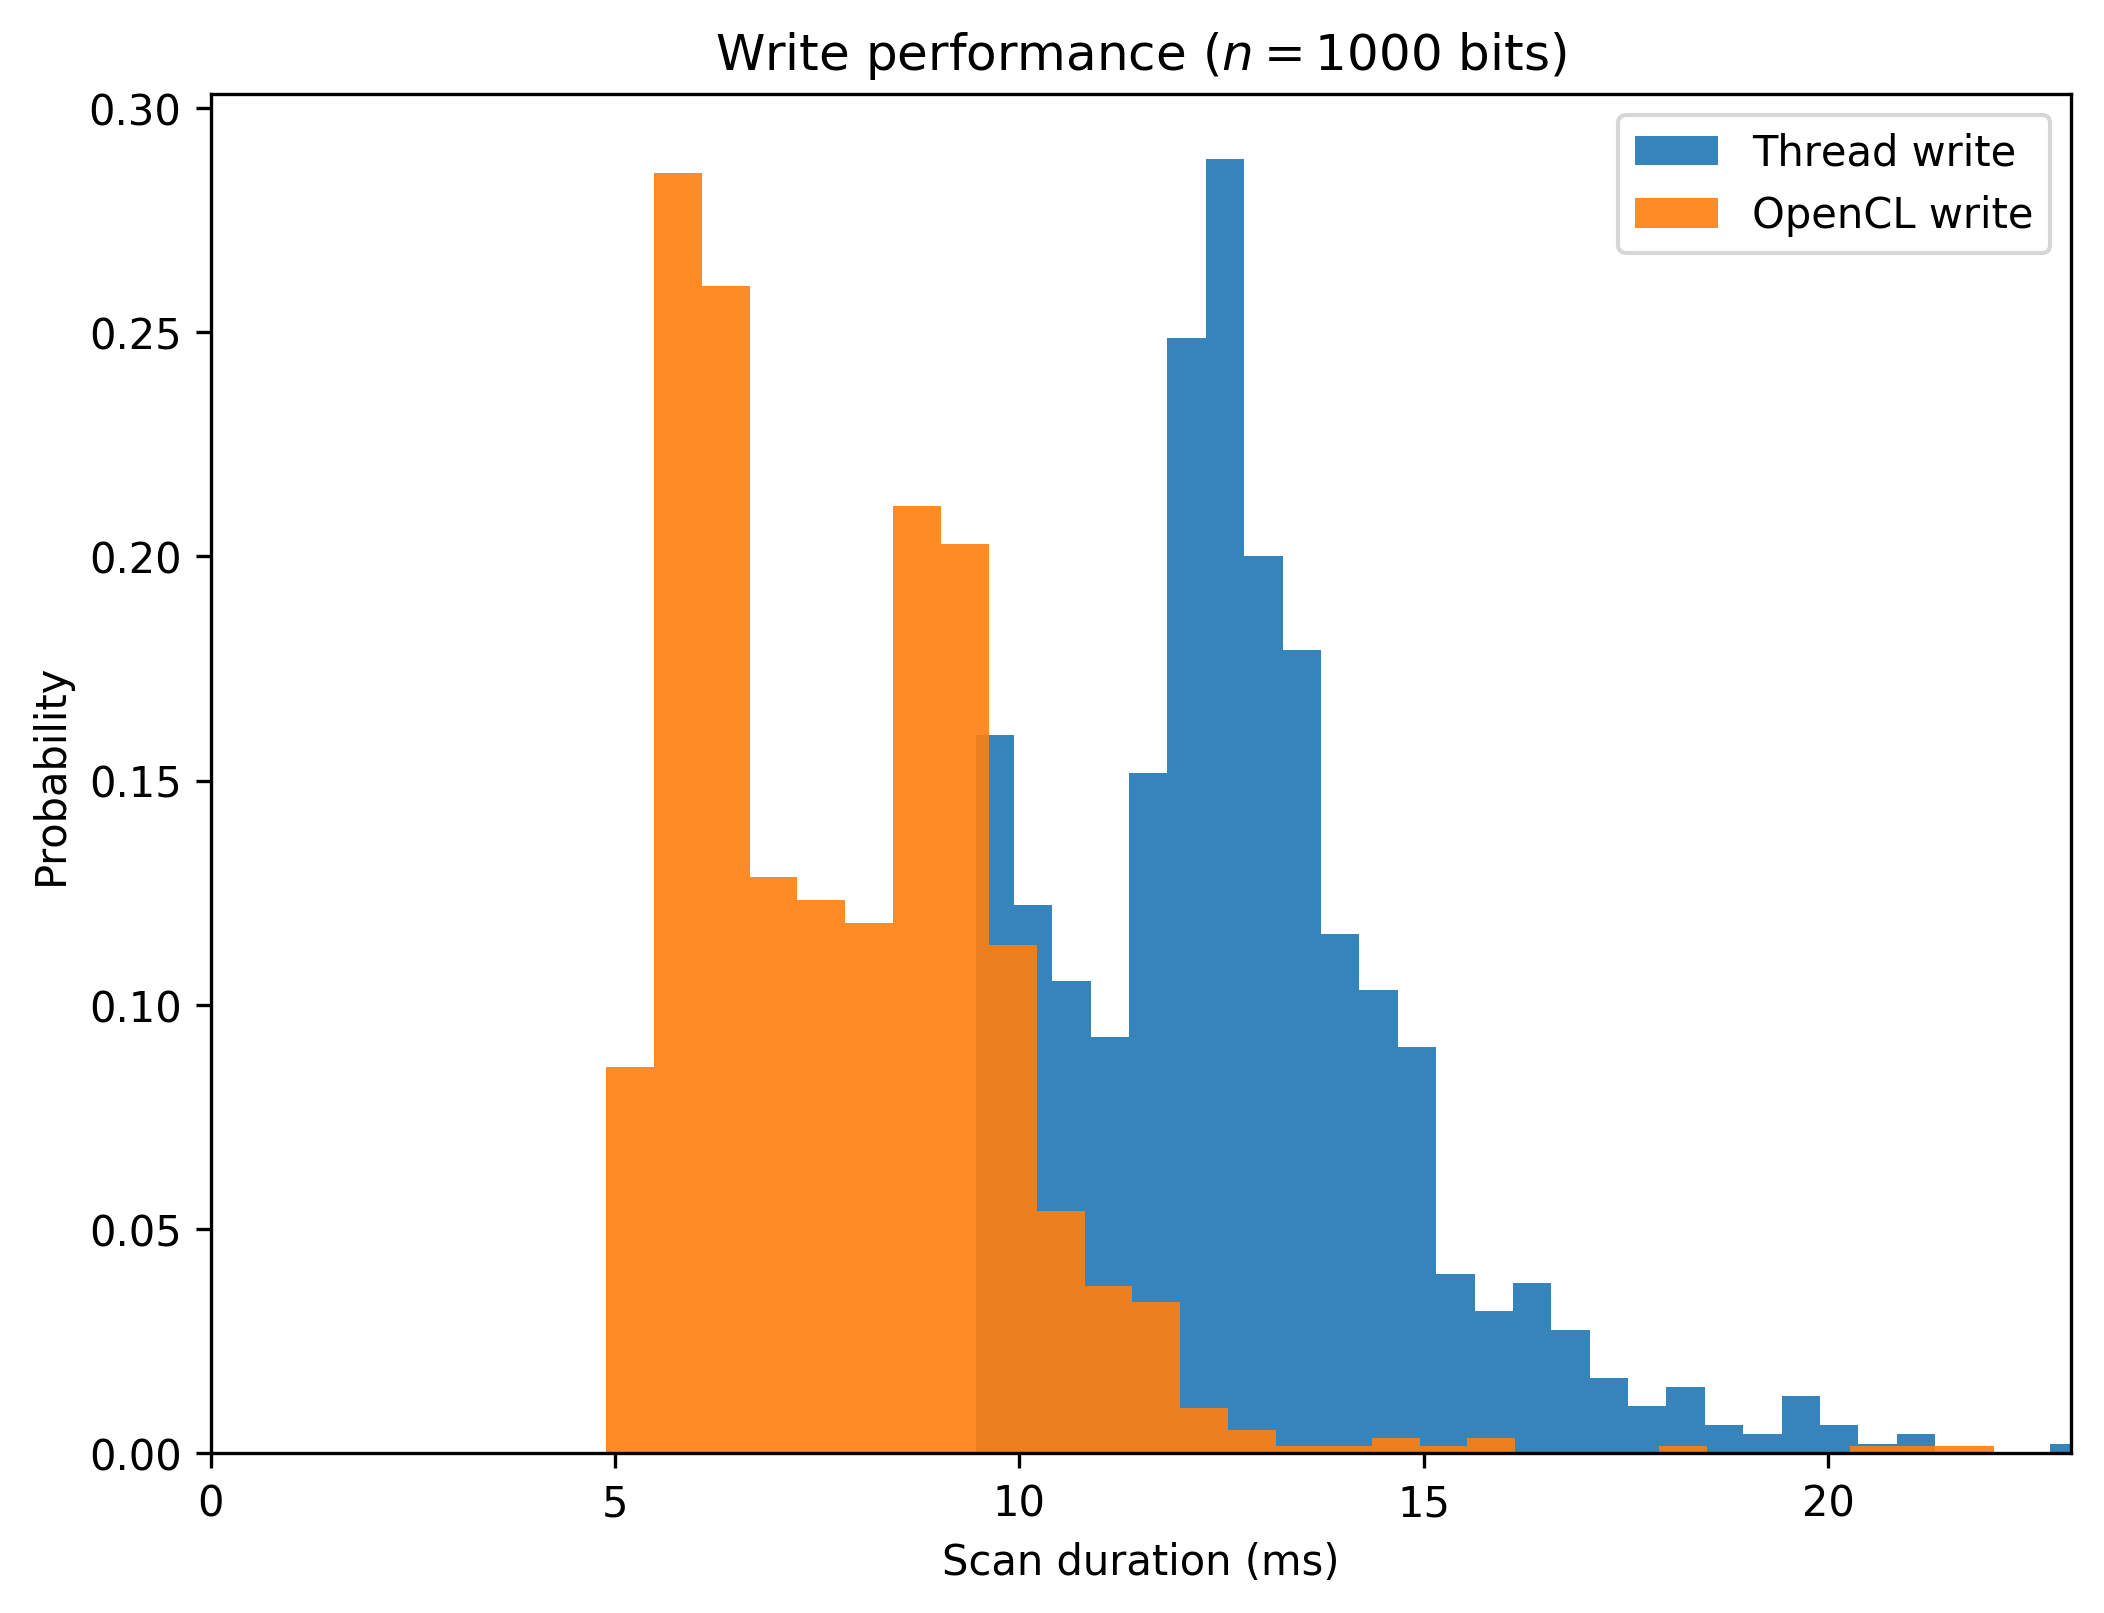
\includegraphics[width=\textwidth]{images02/performance/imac-write-1000.png}
\caption{Time to run one write in a SDM with $n=1,000$, $H=1,000,000$ and $r=451$.
\label{fig:perf-imac-write-1000}}
\end{figure}

\begin{figure}[!htb]
\centering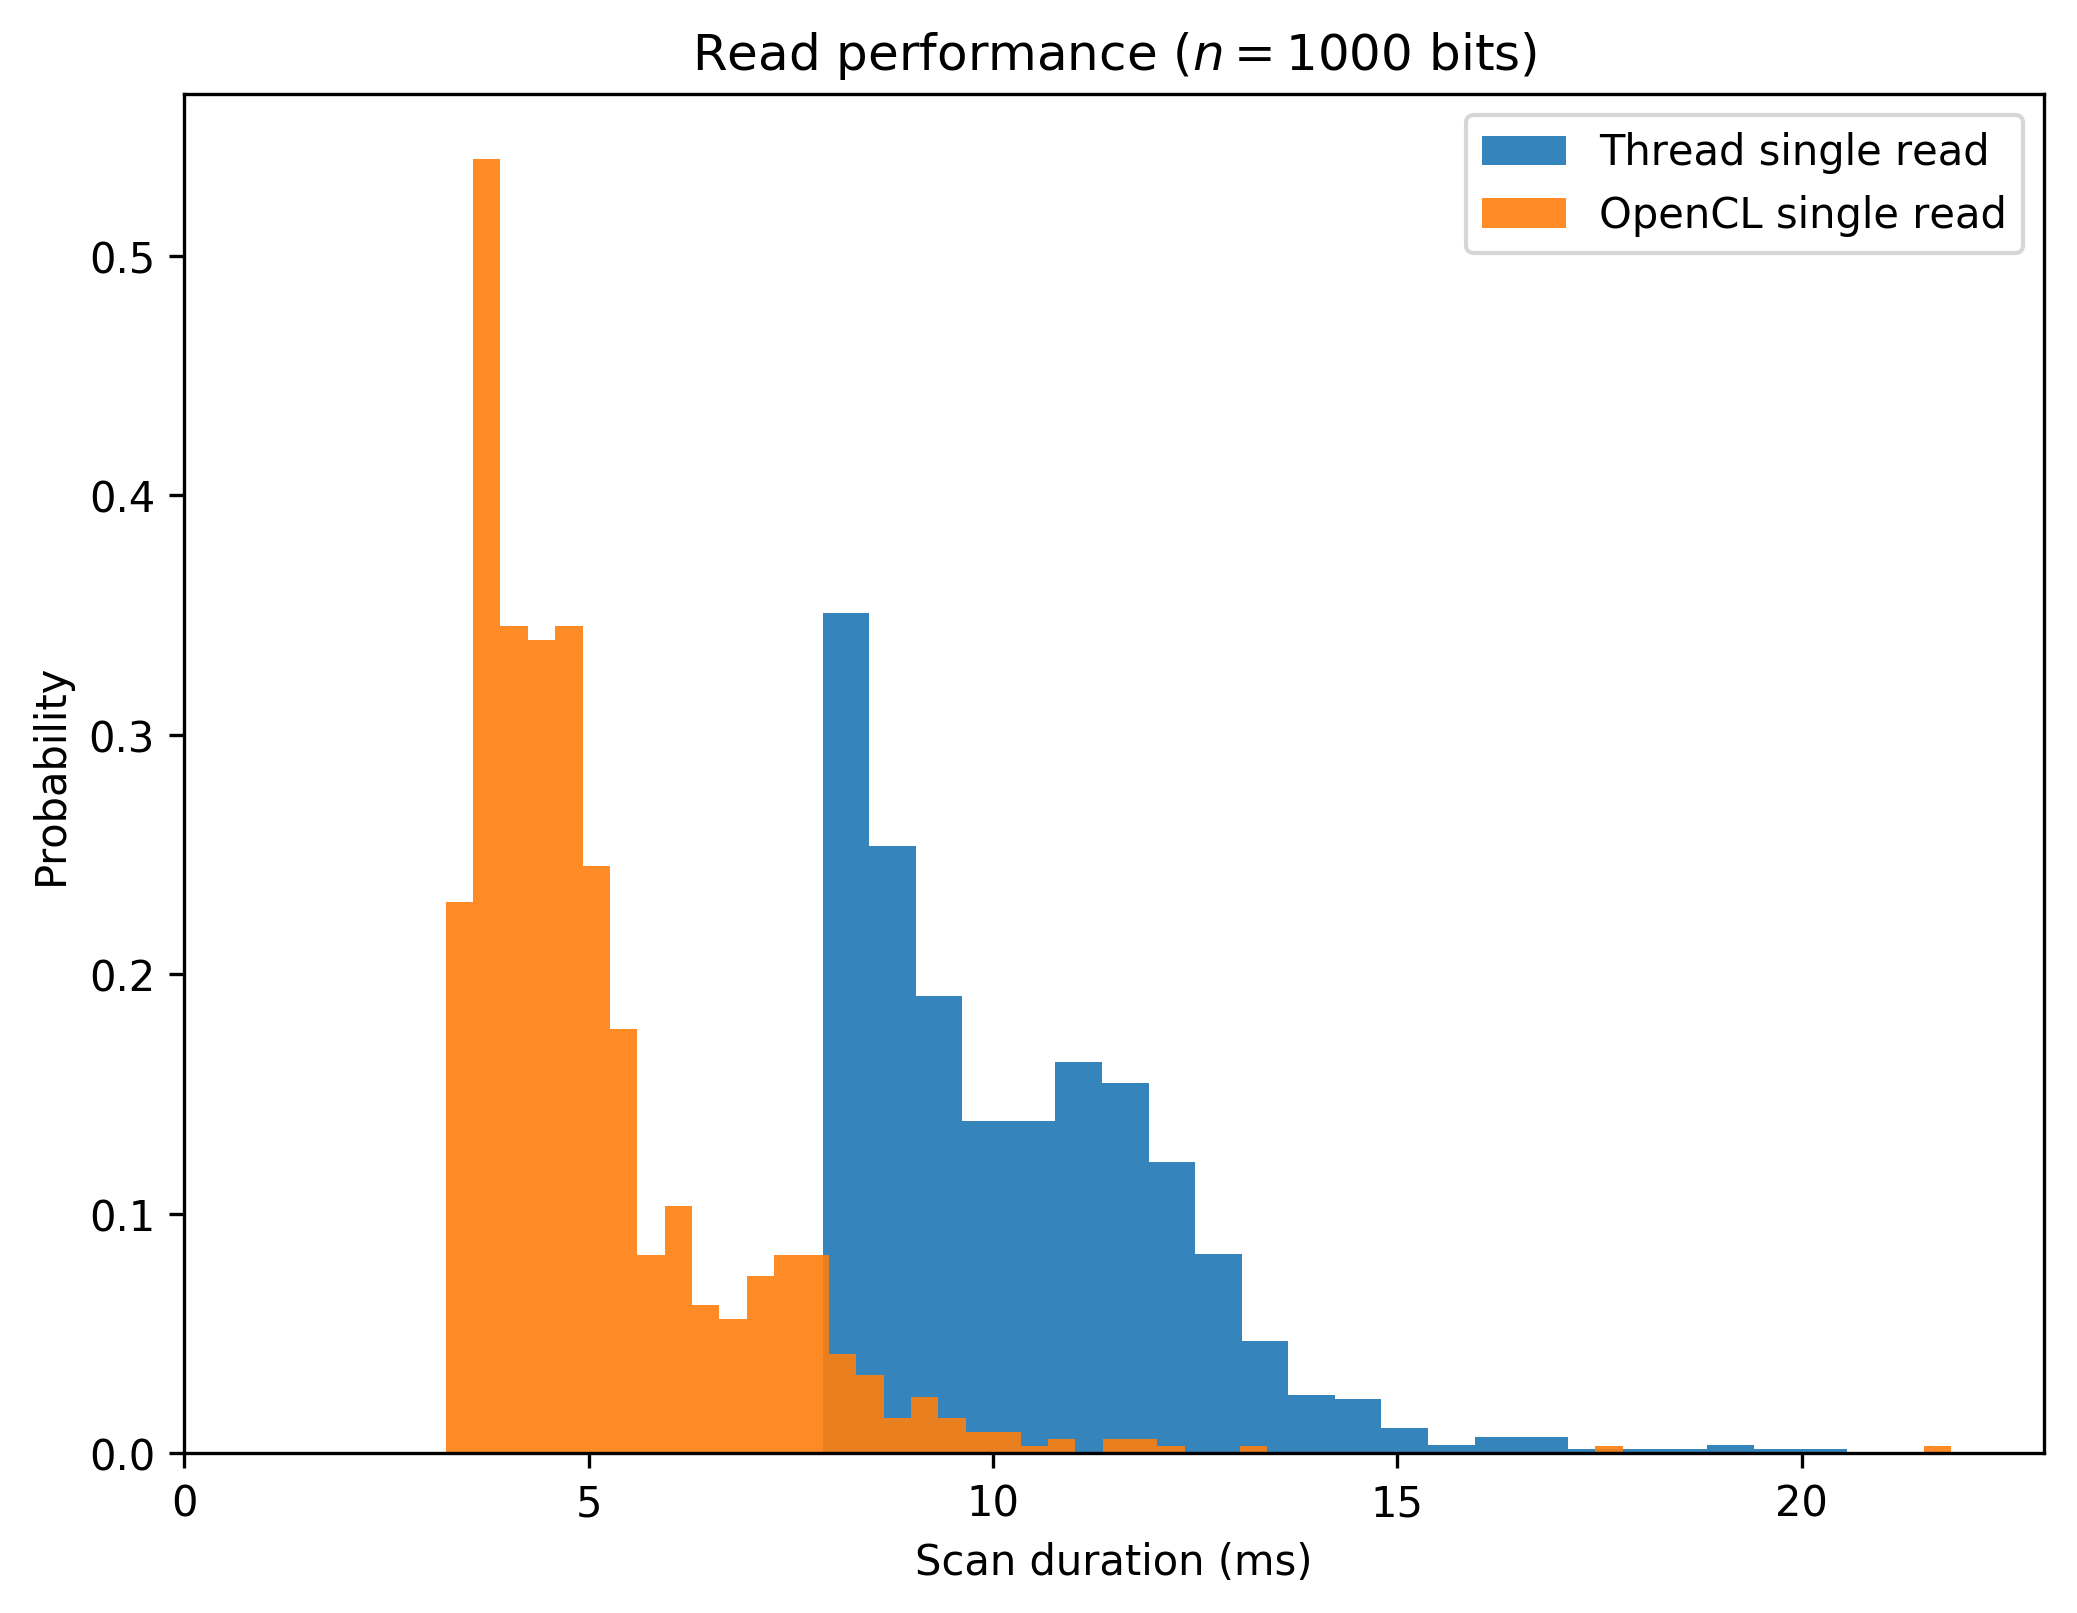
\includegraphics[width=\textwidth]{images02/performance/imac-read-1000.png}
\caption{Time to run a single read in a SDM with $n=1,000$, $H=1,000,000$ and $r=451$.
\label{fig:perf-imac-read-1000}}
\end{figure}

\begin{figure}[!htb]
\centering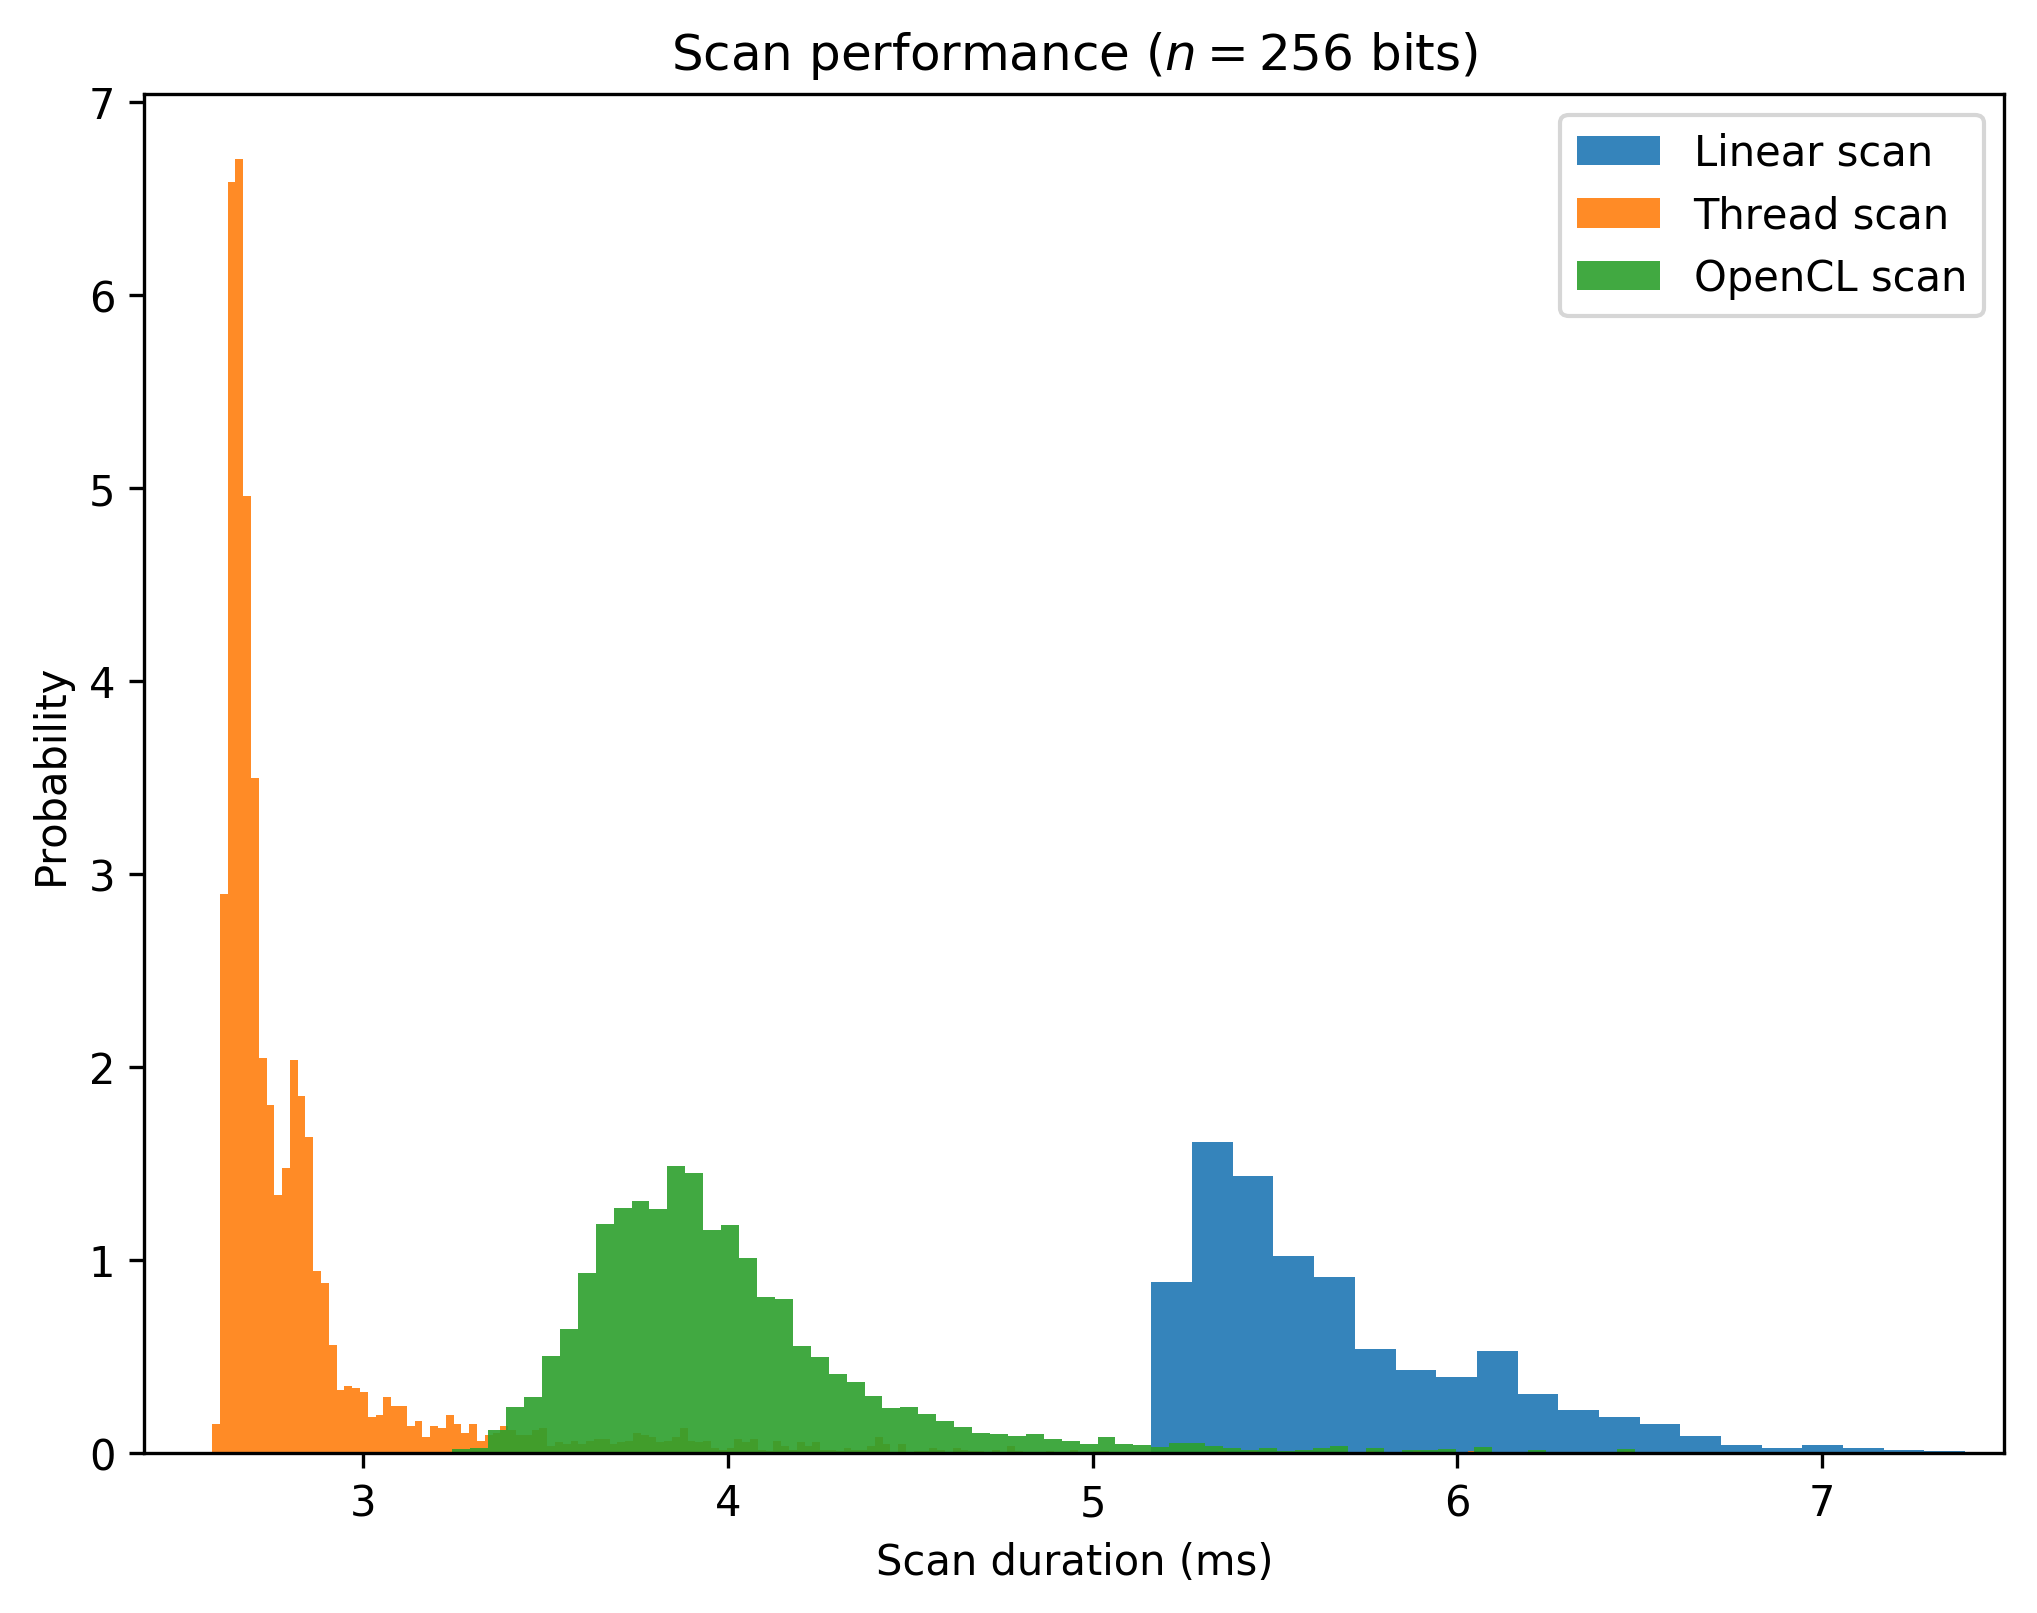
\includegraphics[width=\textwidth]{images02/performance/imac-scans-256.png}
\caption{Time to run a single scan in a SDM with $n=256$, $H=1,000,000$ and $r=103$.
\label{fig:perf-imac-scan-256}}
\end{figure}

\begin{figure}[!htb]
\centering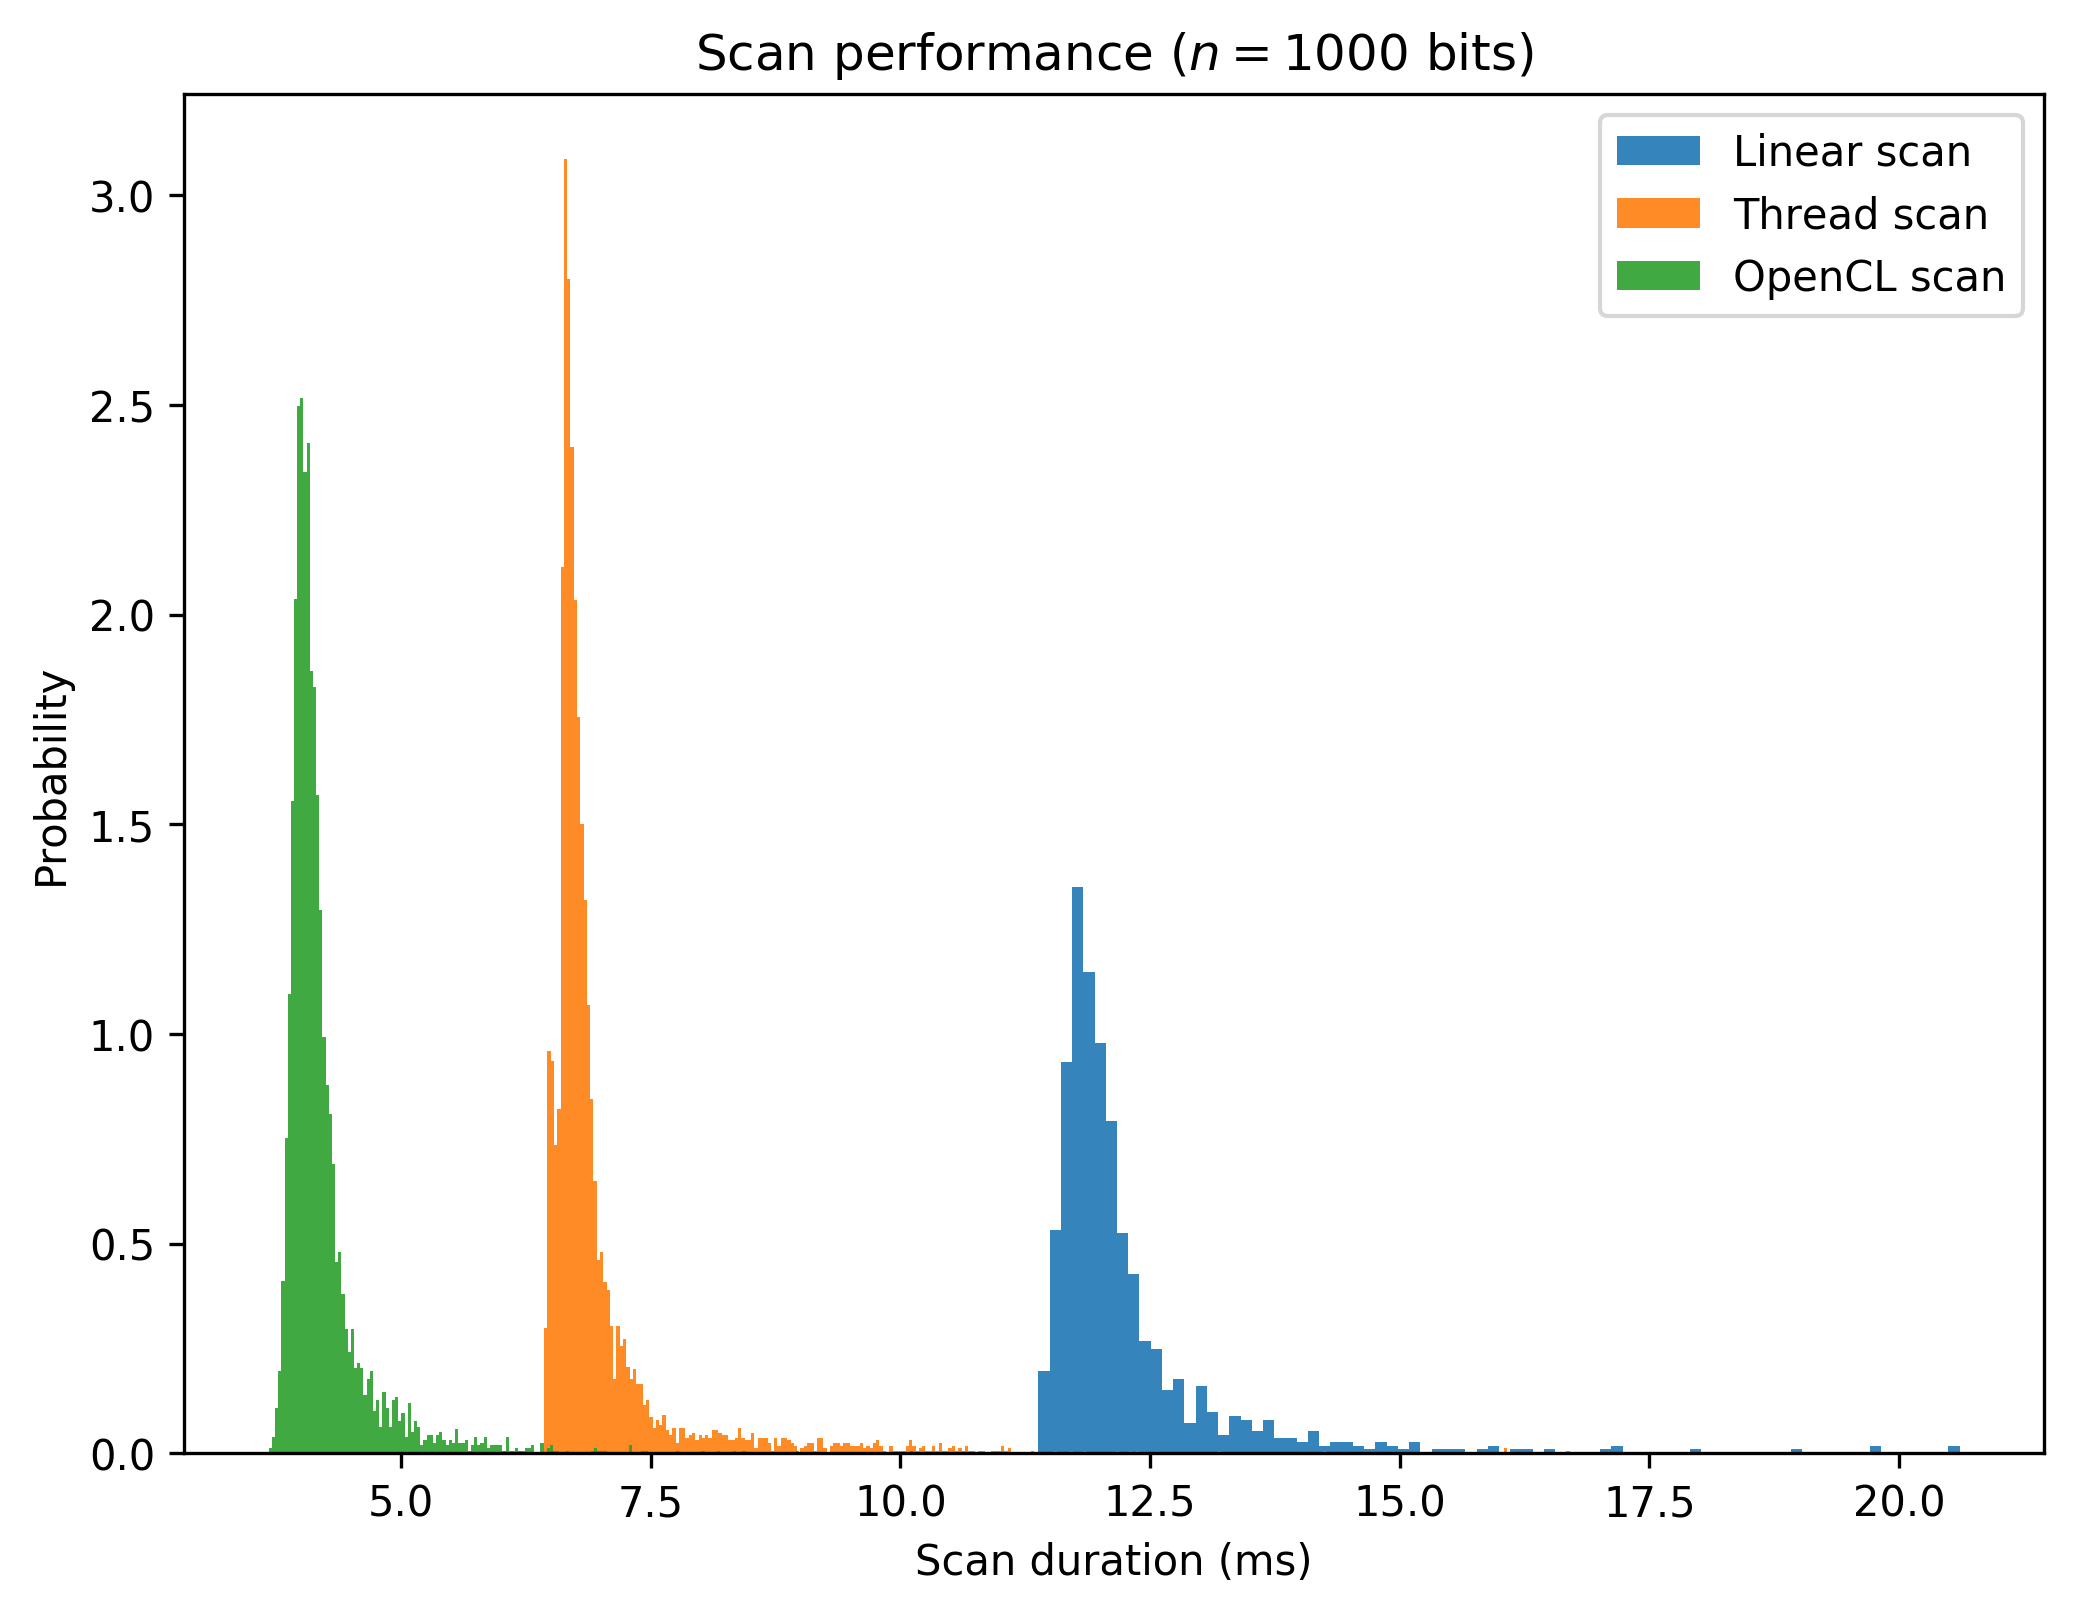
\includegraphics[width=\textwidth]{images02/performance/imac-scans-1000.png}
\caption{Time to run a single scan in a SDM with $n=1,000$, $H=1,000,000$ and $r=451$.
\label{fig:perf-imac-scan-1000}}
\end{figure}

\begin{figure}[!htb]
\centering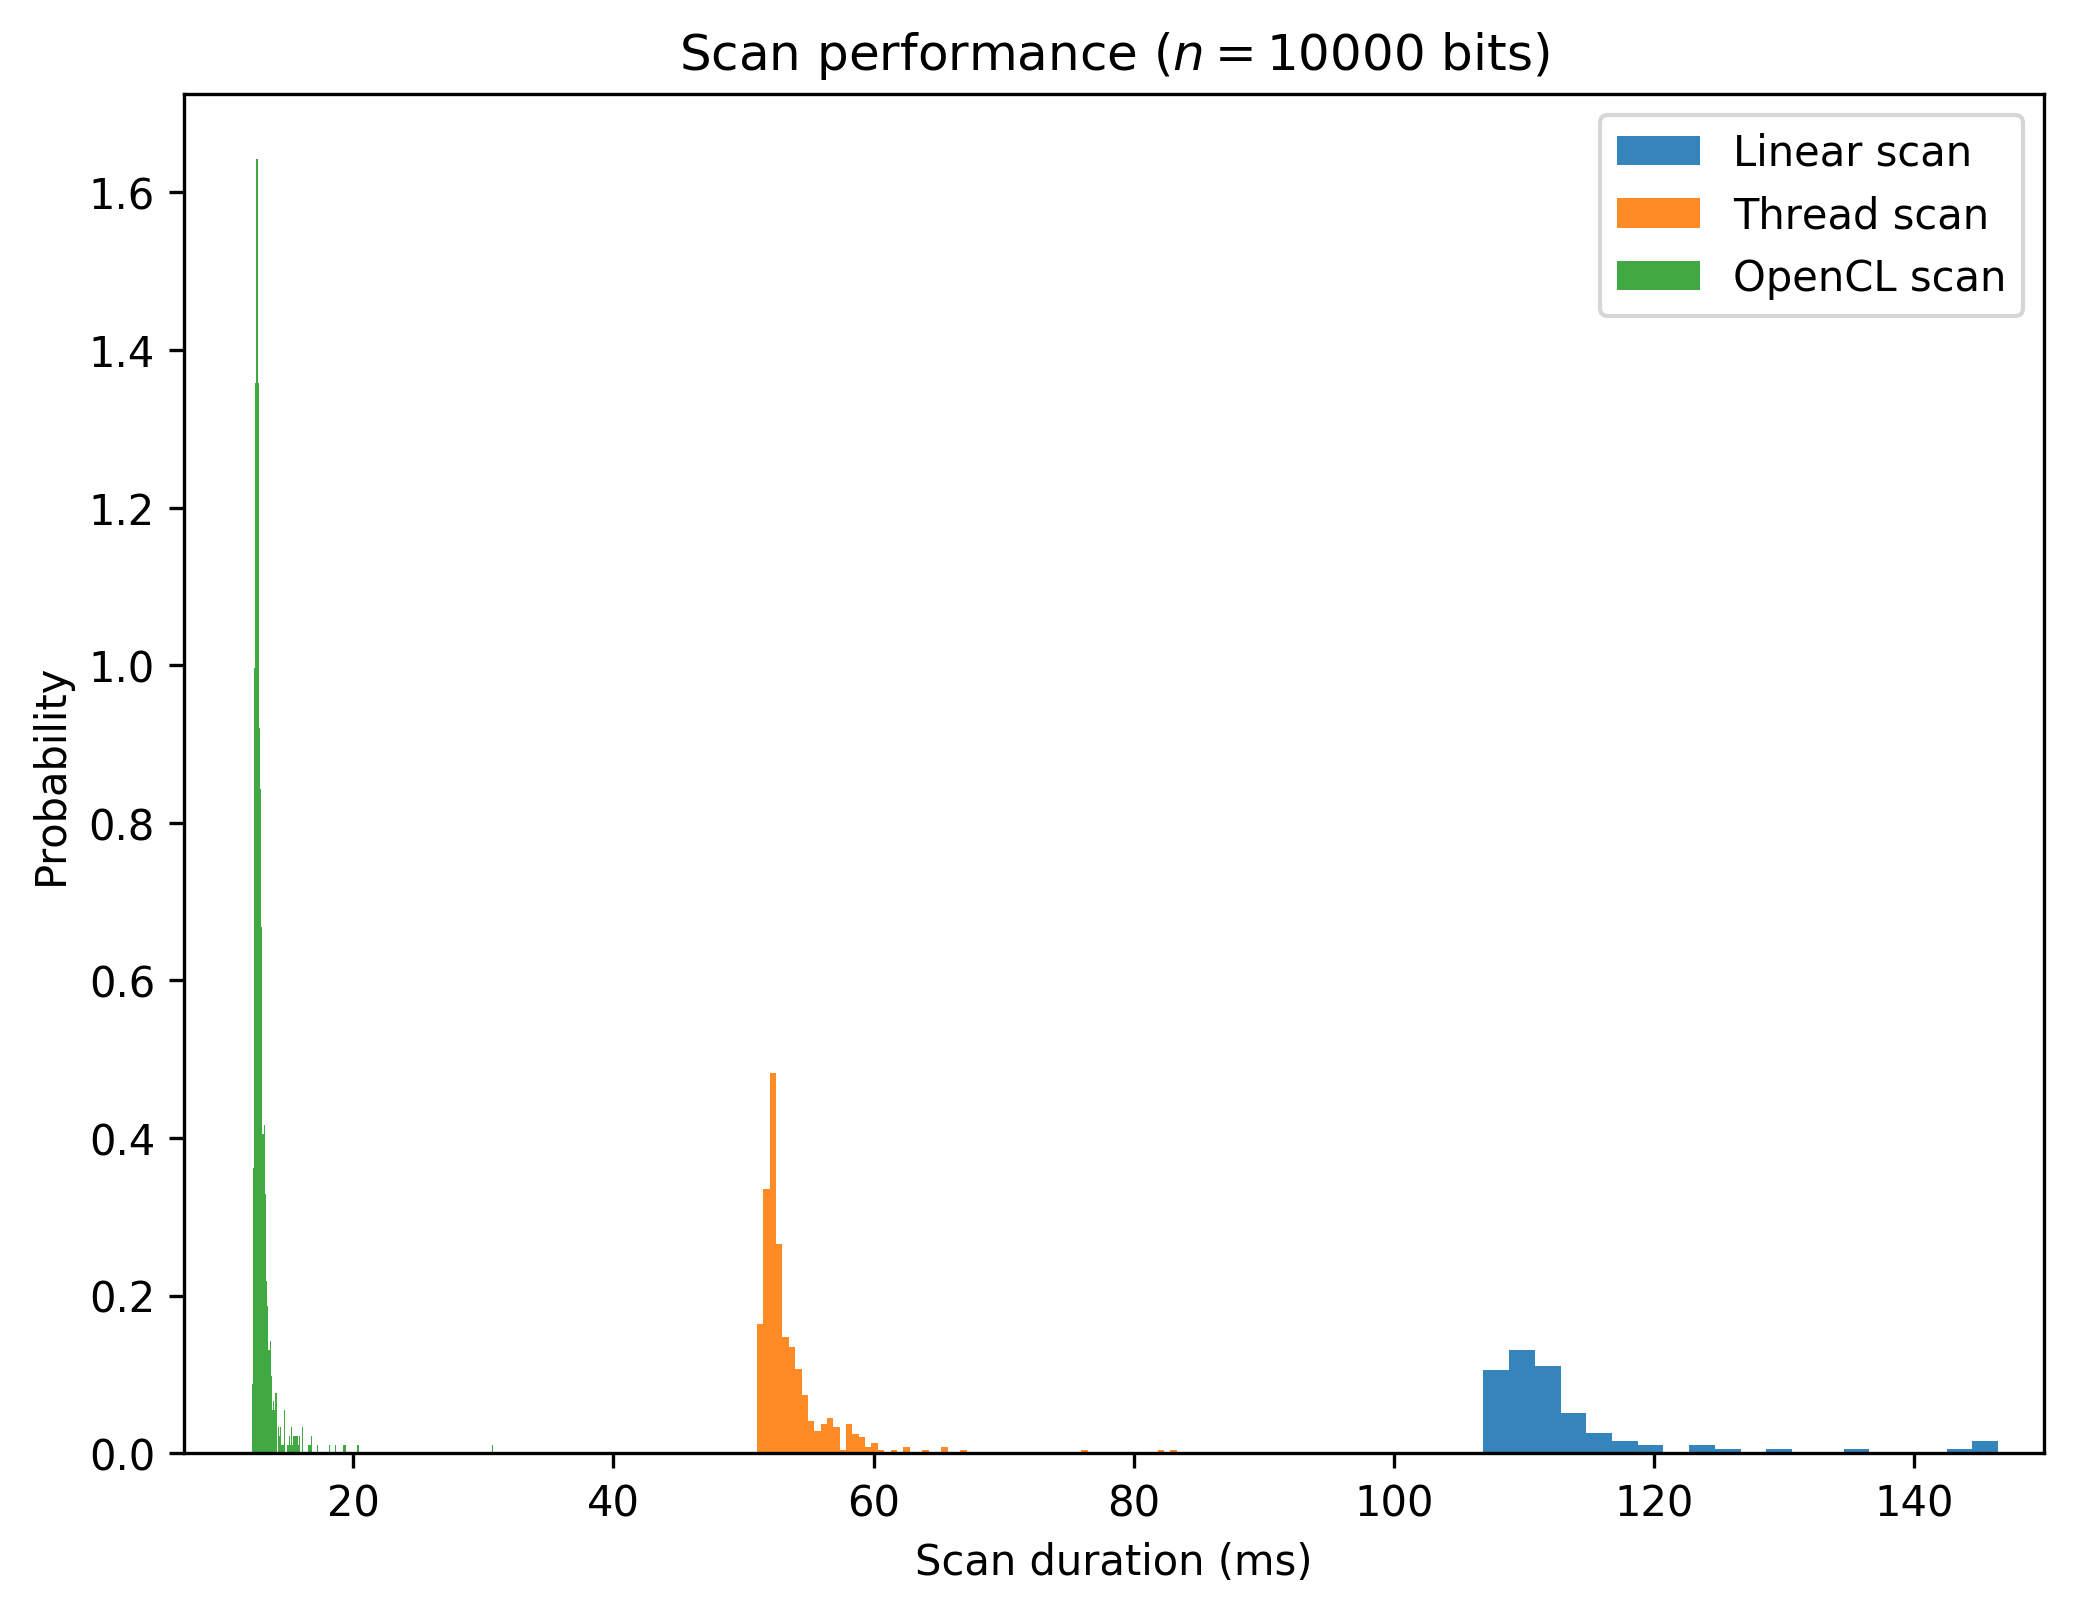
\includegraphics[width=\textwidth]{images02/performance/imac-scans-10k.png}
\caption{Time to run a single scan in a SDM with $n=10,000$, $H=1,000,000$ and $r=4845$.
\label{fig:perf-imac-scan-10k}}
\end{figure}

\begin{table}[!htb]
\centering
\begin{tabular}{| l | r | r | r |}
    \hline
    & Loops & Scans / second & Scan time (ms) \\ \hline
    Linear scan & 1000 & 81.62 & 12.25 \\
    Thread scan & 5000 & 143.68 & 6.95 \\
    OpenCL scan & 5000 & 238.00 & 4.20 \\ \hline
    \hline
    & Loops & Ops / second & Op. time (ms) \\ \hline
    Thread write & 1000 & 74.92 & 13.34 \\
    Thread single read & 1000 & 96.22 & 10.39 \\
    OpenCL write & 1000 & 126.50 & 7.90 \\
    OpenCL single read & 1000 & 190.20 & 5.25 \\
    \hline
\end{tabular}
\caption{iMac Retina 5K 27-inch 2017 with a 3.8GHz Intel core i5 processor, 8GB DDR4 RAM, and a Radeon Pro 580 8G GPU. Running an SDM with $n=1,000$ bits, $H=1,000,000$, and $r=451$.
\label{tab:perf-imac-1000}}
\end{table}

\begin{table}[!htb]
\centering
\begin{tabular}{| l | r | r | r |}
    \hline
    & Loops & Scans / second & Scan time (ms) \\ \hline
    Linear scan & 1000 & 175.48 & 5.69 \\
    Thread scan & 5000 & 352.63 & 2.83 \\
    OpenCL scan & 5000 & 244.88 & 4.08 \\ \hline
    \hline
    & Loops & Ops / second & Op. time (ms) \\ \hline
    Thread write & 2000 & 304.46 & 3.28 \\
    Thread single read & 2000 & 391.21 & 2.55 \\
    OpenCL write & 2000 & 378.44 & 2.64 \\
    OpenCL single read & 2000 & 466.16 & 2.14 \\
    \hline
\end{tabular}
\caption{iMac Retina 5K 27-inch 2017 with a 3.8GHz Intel core i5 processor, 8GB DDR4 RAM, and a Radeon Pro 580 8G GPU. Running an SDM with $n=256$ bits, $H=1,000,000$, and $r=103$.
\label{tab:perf-imac-256}}
\end{table}

\begin{table}[!htb]
\centering
\begin{tabular}{| l | r | r | r |}
    \hline
    & Loops & Scans / second & Scan time (ms) \\ \hline
    Linear scan & 100 & 8.59 & 116.38 \\
    Thread scan & 500 & 18.66 & 53.56 \\
    OpenCL scan & 1000 & 77.20 & 12.95 \\
    \hline
\end{tabular}
\caption{iMac Retina 5K 27-inch 2017 with a 3.8GHz Intel core i5 processor, 8GB DDR4 RAM, and a Radeon Pro 580 8G GPU. Running an SDM with $n=10,000$ bits, $H=1,000,000$, and $r=4845$.  There is no benchmark for read and write operations because RAM is not enough to allocate the counters --- it would consume 37.25 GB of RAM.
\label{tab:perf-imac-10k}}
\end{table}
